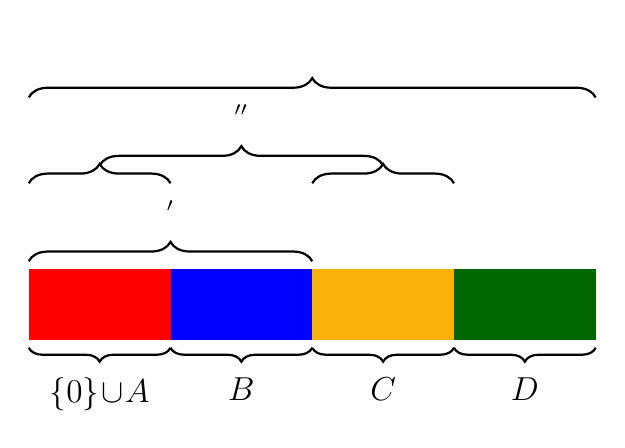
\begin{tikzpicture}[xscale=0.9,yscale=-0.9]

\fill[red] (0,0) rectangle ++(2,1);
\fill[blue] (2,0) rectangle ++(2,1);
\fill[yellow!40!orange] (4,0) rectangle ++(2,1);
\fill[green!40!black] (6,0) rectangle ++(2,1);

\draw [
    thick,
    decoration={
        brace,
		%mirror,
		amplitude=7pt,
        raise=0.1cm
    },
    decorate
] (0,0) -- (4,0)
node  [pos=0.5,anchor=north,yshift=1cm] {$\cC'$}; 

\draw [
    thick,
    decoration={
        brace,
		%mirror,
		amplitude=7pt,
        raise=0.1cm
    },
    decorate
] (1,-1.35) -- (5,-1.35)
node  [pos=0.5,anchor=north,yshift=1cm] {$\cC''$}; 
\draw [
    thick,
    decoration={
        brace,
		%mirror,
		amplitude=7pt,
        raise=0.1cm
    },
    decorate
] (0,-1.1) -- (2,-1.1);
\draw [
    thick,
    decoration={
        brace,
		%mirror,
		amplitude=7pt,
        raise=0.1cm
    },
    decorate
] (4,-1.1) -- (6,-1.1);

\draw [
    thick,
    decoration={
        brace,
		%mirror,
		amplitude=7pt,
        raise=1.1cm
    },
    decorate
] (0,-1.2) -- (8,-1.2)
node  [pos=0.5,anchor=north,yshift=2cm] {$\cC$};


\draw [
    thick,
    decoration={
        brace,
        mirror,
		amplitude=5pt,
        raise=1cm
    },
    decorate
] (4,0) -- (6,0)
node [pos=0.5,anchor=north,yshift=-1.25cm] {\large $C$}; 

\draw [
    thick,
    decoration={
        brace,
        mirror,
		amplitude=5pt,
        raise=1cm
    },
    decorate
] (6,0) -- (8,0)
node [pos=0.5,anchor=north,yshift=-1.25cm] {\large $D$}; 

\draw [
    thick,
    decoration={
        brace,
        mirror,
		amplitude=5pt,
        raise=1cm
    },
    decorate
] (2,0) -- (4,0)
node [pos=0.5,anchor=north,yshift=-1.25cm] {\large $B$}; 

\draw [
    thick,
    decoration={
        brace,
		mirror,
		amplitude=5pt,
        raise=1cm
    },
    decorate
] (0,0) -- (2,0)
node [pos=0.5,anchor=north,yshift=-1.25cm] {\large $\{0\} \!\cup\! A$}; 
\end{tikzpicture}